\documentclass[tikz,border=8pt]{standalone}
\usepackage{amsmath}
\usetikzlibrary{arrows.meta,positioning,fit,calc}

\begin{document}
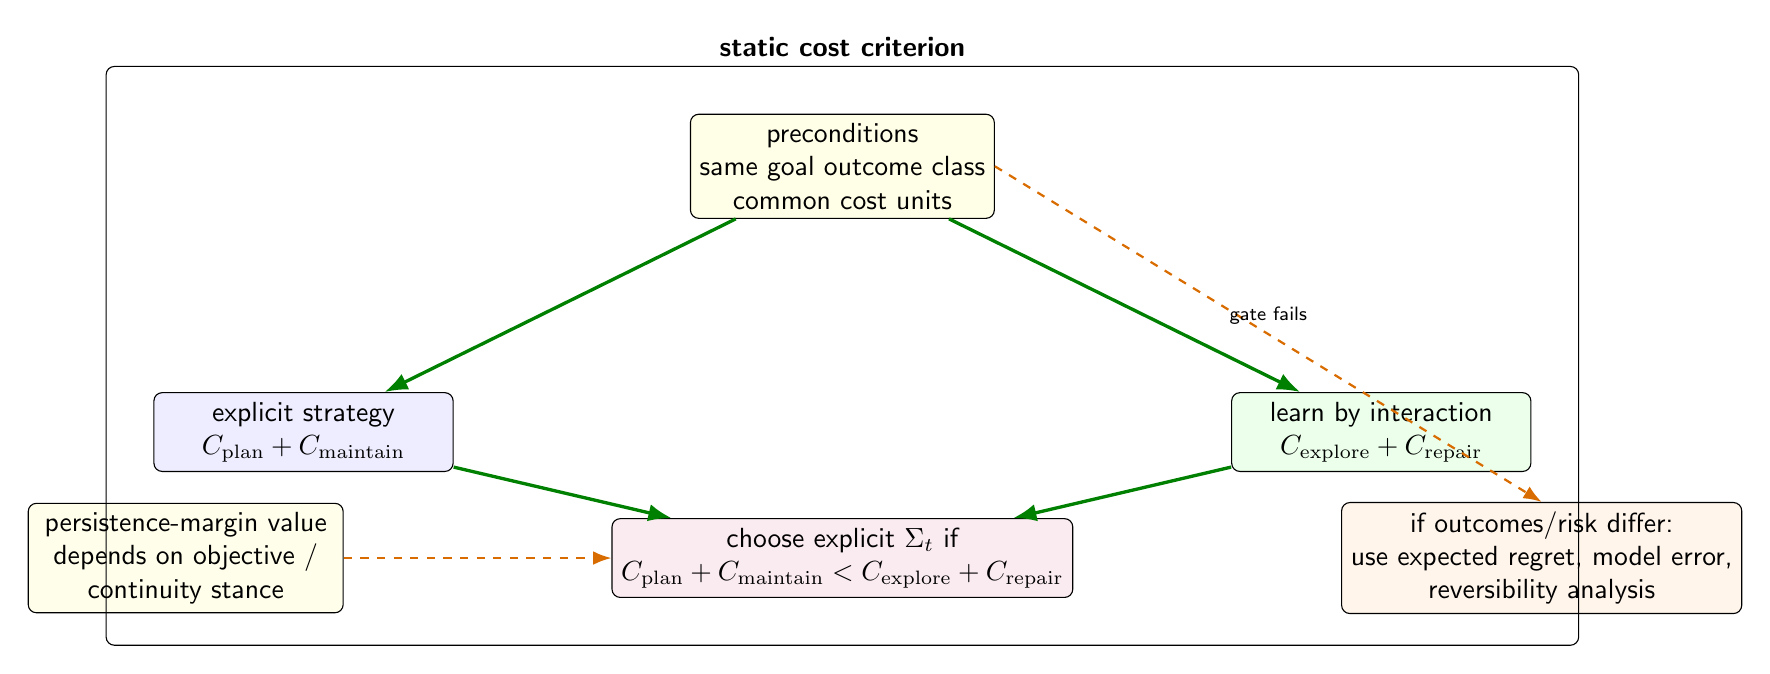
\begin{tikzpicture}[
  font=\sffamily,
  box/.style={draw, rounded corners=3pt, align=center, minimum width=38mm, minimum height=10mm, fill=white},
  small/.style={draw, rounded corners=3pt, align=center, minimum width=28mm, minimum height=8mm, fill=white, font=\sffamily\scriptsize},
  arrow/.style={-Latex, thick, draw=black!65},
  good/.style={-Latex, very thick, draw=green!50!black},
  warn/.style={-Latex, thick, dashed, draw=orange!85!black},
  note/.style={align=center, font=\sffamily\scriptsize}
]

\node[box, fill=yellow!10] (gate) {preconditions\\same goal outcome class\\common cost units};
\node[box, below left=22mm and 30mm of gate, fill=blue!7] (plan)
  {explicit strategy\\$C_{\rm plan}+C_{\rm maintain}$};
\node[box, below right=22mm and 30mm of gate, fill=green!8] (explore)
  {learn by interaction\\$C_{\rm explore}+C_{\rm repair}$};
\node[box, below=38mm of gate, fill=purple!8, minimum width=55mm] (decision)
  {choose explicit $\Sigma_t$ if\\$C_{\rm plan}+C_{\rm maintain}<C_{\rm explore}+C_{\rm repair}$};

\draw[good] (gate) -- (plan);
\draw[good] (gate) -- (explore);
\draw[good] (plan) -- (decision);
\draw[good] (explore) -- (decision);

\node[box, right=34mm of decision, fill=orange!8, minimum width=43mm] (fallback)
  {if outcomes/risk differ:\\use expected regret, model error,\\reversibility analysis};
\draw[warn] (gate.east) -- node[above, note] {gate fails} (fallback.north);

\node[box, left=34mm of decision, fill=yellow!8, minimum width=40mm] (stance)
  {persistence-margin value\\depends on objective /\\continuity stance};
\draw[warn] (stance) -- (decision);

\node[draw, rounded corners=3pt, fit=(gate)(plan)(explore)(decision), inner sep=6mm,
  label={[font=\sffamily\bfseries]above:static cost criterion}] {};

\end{tikzpicture}
\end{document}
